
\chapter{人脸多属性属性识别的架构}
本章主要介绍人脸属性识别任务数据库和一些人脸属性识别中常用的方法,并且根据这些方法的弱点和问题,提出改进方法改进并进行实验。包括人脸属性中输入图片对于识别效果的影响,改进网络结构对于属性性能的提升,设计面向多数据分布和多属性分类的神经网络框架、以及对于网络输出置信度模块的构建。

\section{人脸属性性质分析}
\subsection{人脸属性的类别}
人脸属性的数据标注的环境各有不同限制性场景和非限制性场景(如固定摄像头拍摄和日常采集的场景),其中标签往往具有很多种表示和性质,比如相对性标注和绝对属性标注(如颜值数据标注之间只有相互的高低,但没有绝对的属性标签)但总体分为有序性与无序性,整体性与局部性等,具体包括:
\begin{enumerate}
\item 无序性:
无序性的属性有两个或两个以上的类别(值),但在类别之间没有内在的顺序。 例如,种族是具有多个类别的名义属性,例如黑色,白色,亚洲等,并且这些值(类别)没有内在排序。;
\item 有序性:有序性的属性具有明确的变量排序。 例如,一个人的年龄,通常从0到100,是不平均的。(实际上,年龄不仅是相互独立的存在,在不同的年龄标签中,具有一定钟形的分布)
\item  整体性:
整体性标签描述了整个人脸的特征,诸如年龄,性别,种族等;
\item 局部性:
和整体性标签相反,局部性描述了部分人脸的特征,例如:尖鼻子,大嘴唇等。
\end{enumerate}
本文中也主要根据上面的人脸属性的性质来设计网络和分析问题。

\subsection{多属性标签表示形式}
在训练的过程中,人脸属性通常以分类或者回归问题的形式出现,但是在多属性识别的任务中,通常使用标签编码或者多标签回归的方式。

方法一:标签编码:
将多属性标签组合进行编码(比如,将一岁亚洲男性标记为001,将一岁非洲男性标记为002等),将多属性问题转化为分类编码问题,也就是单一属性。

方法二:多标签回归
通过回归的方法,使预测的特征向量与Groud-truth属性向量的损失越来越小,二者趋向接近,由此得到预测的特征向量。

\subsection{属性之间的相互联系}
正如上文提到的,属性之间具有非常大的异构性,但是作为人脸特征,它们同时在很多表现过程之中,也有很多共同的地方,那么在设计的过程中我们更倾向于用的是单框架多任务方式。这也利用属性之间的相关性,包括正相关和负相关等来进行互相补足;同时多任务的方式设计也应对属性之间的异质性,比如年龄是可量化的,而种族是类别化的,这就需要不同的处理方式。
我们对CelebA数据集的40个属性做了成对的co-occurrence计算,它揭示了,属性的相关性是普遍存在的,且我们认为它对属性学习有所帮助。
\begin{figure}[!ht]
 \centering
	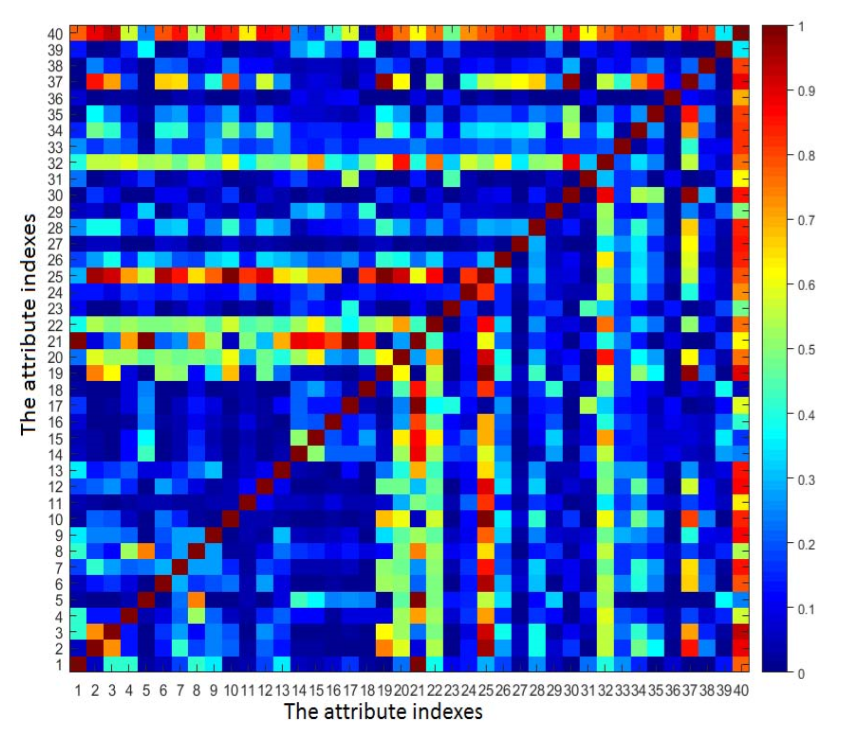
\includegraphics[width=6.0in]{attrconv.png}
	\caption{基于共享神经网络特征和SVM分类器的人脸属性识别}
\end{figure}

\section{人脸属性数据库简介}
这一章主要对于对于具体的数据库进行介绍:
\textbf{MOROH II:}MORPH是一个大型的mugshot图像数据库,每个数据库都有相关的元数据,包含三个标注属性:年龄(有序),性别(无序)和种族(无序)。通过调查MORPH Album II(MORPH II)上的所有三个属性估计任务,其中包含大约78K的超过20K个主题的图像。在MORPH II上的结果五等分数据进行交叉验证。

\textbf{CelebA:}CelebA是一个大型的人脸属性数据库拥有超过10万个身份的200K个名人图像,每个人拥有40个属性注释。该数据集中的图像在姿态,表情,种族,背景等方面存在较大的变化,使得面部属性估计具有挑战性。此外,由于有40个属性标注,CelebA数据库在特征学习效率方面对联合属性估计算法提出了挑战。

 \begin{table}
  \centering
   \caption{celeA中的属性表}
   \label{tab:req-pkg}
   \begin{tabular}{c|c|c|c}
     \toprule
     属性序号 & 属性 &属性序号 & 属性 \\
     \midrule
     |1|  & 5OClockShadow		 & |21| & GrayHair \\
     |2|  & Male 				 		 & |22| & Sideburns \\
     |3|  & ArchedEyebrows  	 & |23| & BigLips \\
     |4|  & MouthSlightlyOpen  & |24| & Smiling \\
     |5|  & BushyEyebrows  		 & |25| & BigNose \\
     |6|  & Mustache           & |26| & StraightHair \\
     |7|  & Attractive         & |27| & Blurry\\   
     |8|  & NarrowEyes 			 & |28| & WavyHair \\
     |9|  & BagsUnderEyes  		 & |29| & Chubby \\  
     |10| & NoBeard            & |30| & WearEarrings\\   
     |11| & Bald               & |31| & DoubleChin  \\
     |12| & OvalFace           & |32| & WearHat \\
     |13| & Bangs              & |33| & Eyeglasses \\
     |14| & PaleSkin           & |34| & WearLipstick \\
     |15| & BlackHair          & |35| & Goatee \\
     |16| & PointyNose         & |36| & WearNecklace \\
     |17| & BlondHair          & |37| & HeavyMakeup\\
     |18| & RecedingHairline 	 & |38| & WearNecktie\\
     |19| & BrownHair          & |39| & HighCheekbones\\
     |20| & RosyCheeks 			 & |40| & Young\\
     \bottomrule
   \end{tabular}
 \end{table}

\textbf{LFWA:}LFWA是另一个无约束的人脸属性数据库,其中包含来自LFW数据库的脸部图像(5,749个主题的13,233张图像),以及与CelebA数据库中相同的40个属性注释。

\textbf{Chalearn LAP and FotW:}ChaLearn挑战系列从2011年开始,在促进人们视觉或多模式分析方面取得了非常成功的成果。LAPAge2015是一个无约束的脸部数据库,用于在ICCV 2015上发布的视在年龄估计。该数据库包含4,699张脸部图像,每个平均年龄至少由10个不同的用户估算。数据库被分割为2,476张图像进行训练,1,136张图像进行验证,1,087张图像进行测试。由于年龄信息的测试不可用,主要使用validation集进行测试。 FotW数据库是通过收集来自互联网的公开可用图像创建的,其中包含两个数据集,一个用于辅助分类,另一个用于性别和微笑分类。 FotW数据集分别包含5,651,2,826和4,086幅用于训练,验证和测试的面部图像; 每个都用七个二进制附件属性注释(见表5(a))。 FotW性别和笑容数据集分别由6171个,3086个和8505个面部图像组成,用于训练,验证和测试; 每个都注明三元性别(男性,女性,不确定)和二元微笑的属性。

\texbf{LBS :}Labeled by self,即实验室自行标注的属性数据集,包括性别,年龄,表情,发型,墨镜等9种属性标注,标签的标准全都是无序性的分类标准,年龄分类标准分成了婴儿,儿童,青年,中年,老年五个类别。一共有8w张图


这些数据库可以根据所使用的注释方法分为三类:(i)具有名义和有序属性的数据库(MORPH II和LFW +),(ii)具有二进制属性的数据库(CelebA,LFWA和FWW)和(iii) 具有单个属性的数据库(LAPAge2015)。 我们可以看到,除了MORPH II数据库,其他数据库主要包含真实场景下的人脸图像。  

可以看到人脸属性的数据集其实比较庞大,如果都能够充分利用,可以获得与使用单一数据集更加出色的识别效果。但是每个数据集之间的数据不同,数量不同,标注不同实际使用中往往使用先训练一个再训练一个的流程,非常耗时而且不能够保证模型效果在原有数据集上保持良好的效果。实际是用来看,使用celeA训练的数据对于lfwA的数据效果并不好,实际上加入lfwA的数据训练就可以提升相关lfwA上的准确率。但需要注意的是LFWA的数据量远小于celeA的数据量,合起来训练,两个数据库之前的差异分布其实并不能得到特别好的弥补,训练的准确率还是不能和单独使用lfwA相比。

类似的问题对于年龄这一属性更严峻一点,不同的数据库标注是不一样的,在morph中是连续的标签,但是在adience数据集上,年龄的标注是7个单独的类别,如果强行进行label的转换就会存在很多不匹配的现象,无法对其进行测试,但根据adience重新finetune,那么就会存在类似的数据匹配和模型输出改变的问题。

\section{基于传统特征的人脸属性识别}
基于传统特征的人脸属性识别往往采用特征提取和分类器结合的方式,其中较为经典的是基于DIF特征的人脸属性识别是经典的属性学习方法,在morphII上一度取得了非常优秀的实验结果,基本框架概述如下:

前端为特征提取阶段,旨在提取对属性有判别力的特征,而不是完全无监督的。后端连接一个层级式的分类器,用于属性学习。具体结构见下图:
\begin{figure}[!ht]
 \centering
	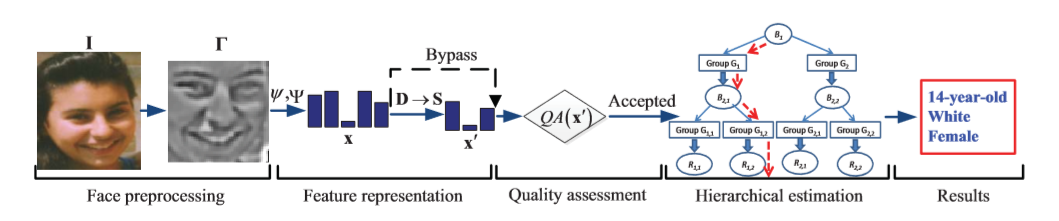
\includegraphics[width=6.0in]{huhanSTLMorph.png}
	\caption{基于DIF特征的人脸属性识别}
\end{figure}

其中有几个主要部分:DIF(Demographic informative features)特征提取,层级式分类器,人机对于单属性预测任务的对比

1)DIF特征:

DIF(Demographic informative features)是基于BIF(生物启发式特征)的。
比如,输入一个人脸部件,先用Gabor滤波器提特征(12个尺度,8个方向),再做一些池化操作,以减小特征图的数目和维度(6个尺度,8个方向),将得到的特征串成一个4280维的长向量,用来做之后的分类等任务。总体上还是一个无监督的特征处理方法。所以之后,又对此工作做了改进,旨在不仅能够抓住图像细节,还能减小冗余性,提高特征与最终识别任务的相关性。这一部分主要引入一些特征学习工作,从之前的特征集中不断特征子集,挑选出最相关的特征,比如:学习一个新的特征子空间(如LDA),基于Boosting的特征选择。

2)层级分类器的建设:

层级分类器主要针对年龄。比如,首先进行年龄组分类(针对数据集设定阈值),在此按是否超过18岁分为两类;低于18岁的一类再判断是否低于7岁,再分为两类,然后低于7岁再进行回归得到具体的年龄数值,以此类推,先一层一层地通过多个分类器树形展开得到具体的人脸年龄段,然后在具体的人连年龄分段中及进行回归。hu的实验证明,这种层级式的分类方式要优于直接分类方法。

基于DIF特征的属性识别方法是经典的基于传统特征和分类器的属性识别方法,即使在现在,特征融合、层级分类器建设等操作依然具有一定的借鉴意义

问题与不足:但存在一定的问题,例如,层级分类器确实能够提升分类的效果,但是复杂都明显过高,并不简洁,使用基于传统滤波器和表层信息的图像特征,需要大量的特征筛选和过滤工作。而且总结来讲是DIF系统还处在各个部分的分开设计,整个系统并不是处在一个整体性学习的状态。需要较多的人工干预和训练才能得到较好的效果。

\section{基于共享神经网络特征和最大间隔分类器的人脸属性识别}
随着深度学习方法的提出,深度学习的特征慢慢取代了传统的手工设计的特征,结合深度学习中经常使用的分类器,得到了更高的效果。
具有代表性的是基于级联CNN网络和SVM分类器的识别方法,使用两个CNN框架Lnet和Anet进行级联学习,其中Lnet负责检测图片中的人脸,Anet针对于Lnet中检测人脸使用交叉熵loss进行训练,为了提升识别的准确性使用SVM对于ANet中的特征进行训练。最后由SVM分类器输出具体的人脸属性预测值。
其中不难发现器图片的标签就采用的是标签化编码的方式。
\begin{figure}[!ht]
 \centering
	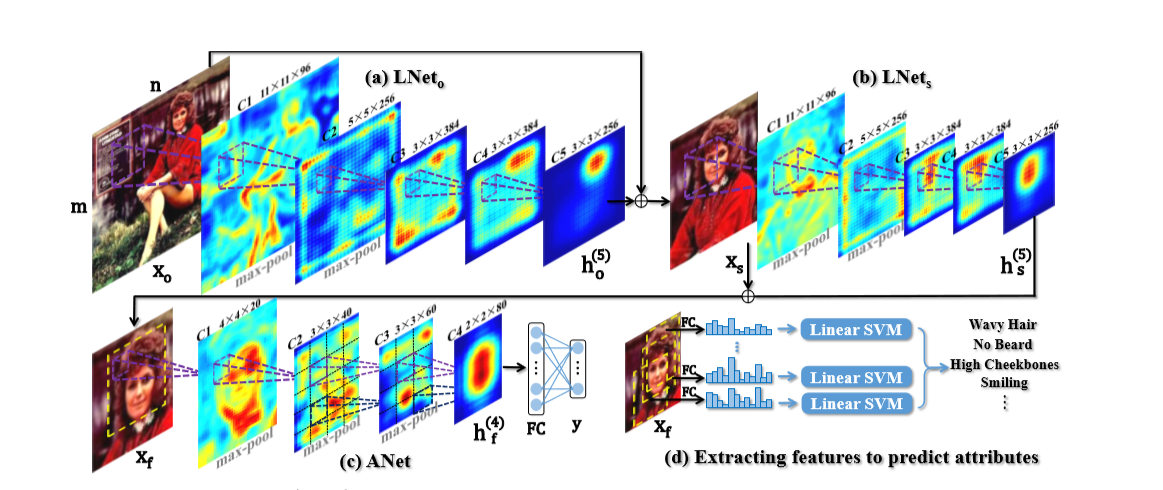
\includegraphics[width=6.0in]{liuziwei.png}
	\caption{基于共享神经网络特征和SVM分类器的人脸属性识别}
\end{figure}

问题与不足:其实在训练的过程中,神经网络就已经可以对于属性进行预测,但是识别的效果却并不如SVM训练的结果,说明在这一框架中,神经网络对于不同属性的自网络决策层和loss函数设计的不够好。从图中可以看到,不同的人脸属性之间都是用的同样的FC层全连接而来的。不能够体现出属性整体和局部特性。
 
\section{基于共享特征和子任务模块的端到端的人脸属性学习}
机器学习神经网络中的端到端,一般是指输入原始数据,输出最后结果的过程。对于人脸属性的识别过程来讲:如何解决人脸属性多任务的输出是解决问题的关键,目前比较主流的方法是使用网络共享单元和网络子任务模块相互组合的方式,具体来讲可以参考下图:
\begin{figure}[!ht]
 \centering
	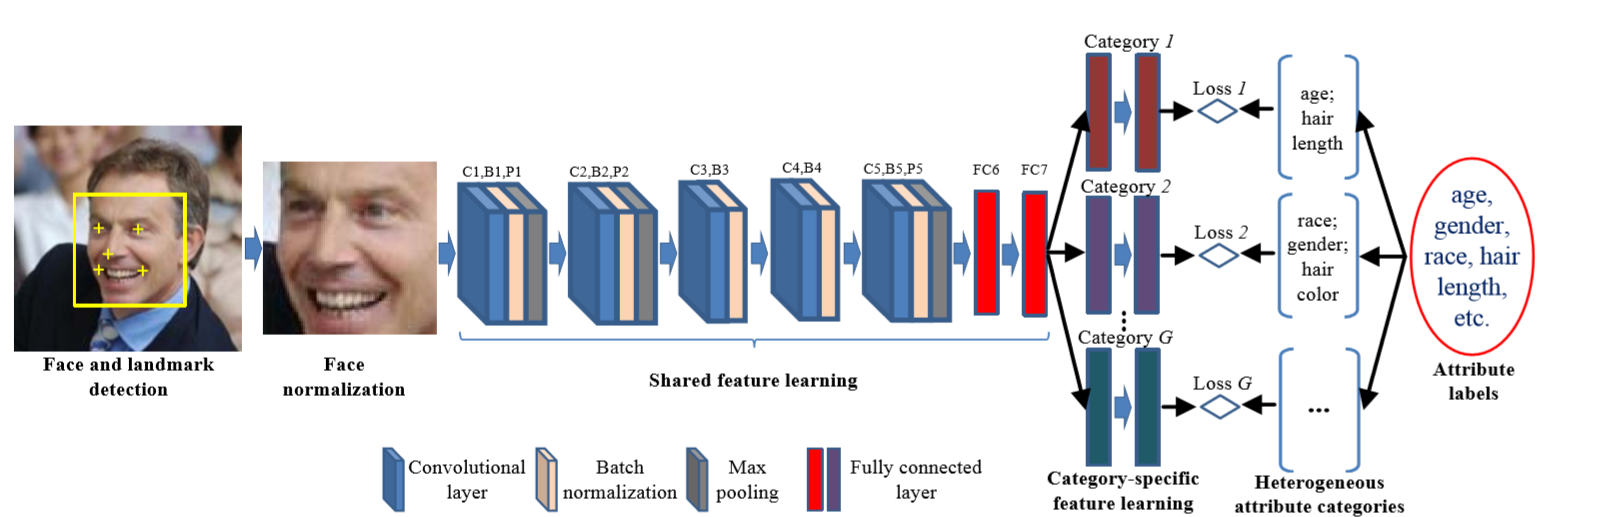
\includegraphics[width=6.0in]{huhanMTL.png}
	\caption{基于端到的人脸属性学习}
\end{figure}
对于不同的人脸识别任务,如果希望能够在一个框架中通过端到端的方式解决,而且具有一定可用性,就需要将不同属性识别任务中重复性学习的工作整合成共享模块,然后不同的人脸属性模块再基于共享模块单独对于自身的学习任务单独进行学习。端到端基于共享模块的学习方法可以很大程度上加快过程中的使用效率,同时简化了训练流程。而类别特定的子模块学习旨在对共享特征进行精细调整,以便对每个异构属性类别进行最优估计。 由于有效的共享特征学习和类别特定的特征学习,基于共享单元和网络子任务模块的方式在保持低计算代价的同时,实现了更高精度的属性估计精度,使其在许多人脸识别应用中具有价值。

问题与不足:基于共享模块和子网模块的识别方式虽然看上去简化了识别的过程,但却是以减少了模型训练的先验规则为代价。也就是说把更多的学习过程交给了模型本身,那么模型的学习过程一方面取决于模型自身设计的学习能力和使用的训练方法,而更重要的是训练数据的选择和实用。

尤其对于端到端网络来讲,由于整体网络结构变得封闭和训练方式的固定化,训练数据的选择和训练过程中对于真实环境的模拟就变得尤为重要。但真实场景中的数据具有较大的变化,包括数据的场景来源不同,数据中样本的比例不均匀,数据自身的姿态和角度变化等。训练样本的选取和预处理过程成了和网络结构选择一样重要的问题。

\section{使用SA-sfotmax进行模型稳定化输出}
模型的稳定性输出体现在很多方面,如常见的连续变化的视频,不同设备收集的图像等。在这些场景中,网络可能偶尔会发生判断错误的情况,影响用户的体验。虽然很多时候可以采用平滑的策略进行弥补,但是网络本身的稳定性性能是整个识别系统的关键。
为了提升属性识别模型的稳定化输出,我提出了基于带有自评功能的softmax(Self-assessment softmax SA-softmax),以及相应的动态标签(Dynamic tag,Dt)训练方法来增强网络的稳定性。
 
\subsection{SA-softmax的改进形式}
传统的softmax with loss 面对N个输入类别,或有N元数字作为输入,同时输入的标签是从0~N-1的一个整形数字用以表示具体的ground truth。通过softmax操作,计算出每个类别的相对概率值。
将对应标签的概率输出取负对数作为损失函数和优化的对象。

SA-softmaxLoss在分类结果上将网络分类概率输出由N个,改为N+1个,第N+1维值定义为无法识别类(unrecognizable class)。

分类label由原来的一元数字标签变为一个四元的整形数组分别用于储存图片在过去训练过程中出现的次数、图像被判正确的次数、图像真实的标签,图像目前的标签。

训练的过程中使用动态标签(Dynamic tag,Dt)训练方法,不断更新训练图片的类别。

测试的过程中,首先使用softmax对于所有N+1类求出无法识别类的概率输出,根据置信度对照表给出网络置信度评价,对其余的类别重新使用softmax进行概率获取。最后的输出形式是:输出类别概率+网络置信度概率。

 \begin{table}
  \centering
   \caption{SA-softmax的置信度判断对照表}
   \label{tab:req-pkg}
   \begin{tabular}{c|c}
     \toprule
     无法识别类概率 & 模型自评置信度 \\
     \midrule
     80-100 & 判定完全无法识别				 	\\
     60-80  & 判定难以识别 				 		\\
     40-60  & 判定可以猜测 但不对结果负责  	 	\\
     20-40  & 判定基本正确    					\\
     0-20   & 判定模型输出非常自信				\\
     \bottomrule
   \end{tabular}
 \end{table}

\subsection{动态调整标签的训练方法}
对于softmax简单的加入一类未知类,还远远不够,至少训练的样本都没有,这分支的梯度永远都是0,不会对网络产生训练作用。但实际上训练开始的时候我们是无法知道哪些图片是网络不能够正确识别的,所以引入动态调整标签的训练方法:
于是在现有的框架下,我们设计了如下的样本生成策略:
步骤一:首先需要在不加入未知类的模式下,将分类网络训练至收敛。

步骤二:将训练收敛的网络模型的softmax改成SA-softmax,即输出的预测类别增加一个未知类

步骤三:正常训练10个epoch,在这个过程之中,每次都更新训练图片的标签四元组中的出现次数和判断正确次数。

步骤四:检查图片现有标签和实际标签是否一致,
如果一致且训练10次准确率高于0.5,那么说明被模型学习的很好,不对标签进行修改;
如果一致但训练10次准确率低于0.5,将图片标签标记成N+1类;
如果不一致且准确率低于0.5,将模型的标签改回原来的标签,看看经过改进的网络能否针对原标签进行拟合;
如果不一致但准确率高于0.5,说明这类图片被成功分到无法识别类,模型认识到自己的局限性。
同时清空出现次数和被判断正确的次数。返回步骤三

\section{实验设置}
在上一节中,总结了在人脸属性任务的主流方法和发展过程,可以看出随着深度学习的发展和端到端学习在模式识别过程中的发展,很多问题都得到了改善,但依然存在着一些主流问题和场景困境一直存在,我仔细对于相关问题进行了思考总结。
\begin{enumerate}
\item 问题1:人脸数据库的标注各不相同,使用怎样的框架才能将不同的数据库都充分利用起来。
\item 问题2:使用怎样的数据输入和数据处理方式和训练方式,才能发挥深度学习的特性。
\item 问题3:提高模型输出的稳定性,减轻网络错误输出的偶然性和影响。
\end{enumerate}
并且根据具体问题设计了实验来改进相关的问题,其中所有的网络结构设计都遵循着神经网络端到端的设计思想,以alexnet为基础进行改进:

\subsection{数据集并行训练的方式改进问题1}
对于不同的数据集来讲,预处理的方式往往类似,也就是说输入图片虽然不同,但是输入的格式是一致的(事实上即使不同也没有什么问题,关键是图片数据不同),但是因为标签不同,导致在一个网络结构中无法进行统一的训练。那么不妨就按照多个单独的网络对于图像进行训练,每个网络在特征提取阶段采用相同参数的全卷及网络结构进行特征提取,但每一层的特征图会单独进行存储,训练的时候每个数据集都按照自己的数据结构特性为了拟合loss层的设计,采用不同的子网络结构。	


(画图)


 \begin{table}
  \centering
   \caption{在LFWA和CELEA上的准确率结果
   \label{tab:req-pkg}
   \begin{tabular}{c|c|c}
     \toprule
          数据集& & 模型自评置信度 \\
          训练集&测试集&40类分类结果的准确率\\
     \midrule
     Morph II & Morph II&            \\
     LBS  & LBS & 判定难以识别            \\
     MorphII+LBS  & Morph II &  判定可以猜测 但不对结果负责      \\
     MorphII+LBS  & LBS & 判定基本正确              \\
     \bottomrule
   \end{tabular}
 \end{table}



\subsection{人脸矫正固定输入格式和数据增强改进问题二}
首先经过图像预测处模块,将图像通过一些基础的图形变换转到统一的形变空间中,常见的操作包括图像识别任务中的空间颜色变换,尺度统一化,多尺度变换,多位置截取等。在人脸属性的人物之中,我们经常采用的方式是人脸alignment,也就是根据人脸检测输出的人脸边框位置和landmark,通过仿射变换,将人脸图像中的关键点映射到图像中的标准位置。
(加入变换公式)


\subsection{网络自评估模块改进问题三}


简单介绍一下人脸矫正的过程:

经过人脸矫正之后,不同的算法和模型其实是对人脸矫正之后的图片或者说一定3*H*W维数值分布在(0-255)的向量空间进行各种线性和非线性计算,最后输出图片对应的属性分类标签的过程。
(加一个简单的流程图)
人脸矫正顾名思义:就是将不够“端正”人脸调整到标准的大小,位置和姿态,这样可以让人脸都在同样的环境下进行比较,人的面部姿态一般会从roll(平面旋转), pitch(左右侧脸)和yaw(抬头低头)三个维度来描述。平面旋转很容易处理,只需将图片旋转一个角度调整至水平即可。而侧脸和低头处理起来比较有挑战,但通过放射变化也可以较好的解决。
在具体介绍人脸属性的任务过程中,首先对于人脸属性的一些常见问题做简单的介绍:
人脸属性识别的输入一般为具体的RGB图片,同时至少带有人脸检测输出的人脸框以及用于人脸矫正的landmark,实际实验证明,经过矫正的人脸对于和人脸姿势无关的属性具有很好的提升。

